\documentclass[conference]{IEEEtran}
% If the IEEEtran.cls has not been installed into the LaTeX system files, 
% manually specify the path to it:
% \documentclass[conference]{../sty/IEEEtran} 
\usepackage[brazil]{babel}
\usepackage{amsmath}
\usepackage{multirow}
\usepackage[utf8]{inputenc}
\usepackage[T1]{fontenc}
\usepackage{graphicx}
\usepackage{adjustbox}
\usepackage{booktabs}

% correct bad hyphenation here
\hyphenation{op-tical net-works semi-conduc-tor IEEEtran}

\begin{document}
	
	% paper title
	\title{Avaliação de Classificadores utilizando Técnicas de Estimativa de Densidades}
	
	
	% author names and affiliations
	% use a multiple column layout for up to three different
	% affiliations
	\author{\authorblockN{Victor São Paulo Ruela \\}
		\authorblockA{Programa de Pós-Graduação em Engenharia Elétrica\\
			Universidade Federal de Minas Gerais\\
			Belo Horizonte, Brasil\\
            Email: victorspruela@ufmg.br}}
	
	% avoiding spaces at the end of the author lines is not a problem with
	% conference papers because we don't use \thanks or \IEEEmembership
	
	% use only for invited papers
	%\specialpapernotice{(Invited Paper)}
	
	% make the title area
	\maketitle
	
	\begin{abstract}
		A modelagem de dados não-lineares com redes neurais artificiais depende da qualidade projeção aplicada sobre as entradas, geralmente feita através de funções de kernel. A otimização de seus parâmetros é uma etapa importante e pode ser feita via técnicas de estimativa de densidade. Além de fornecer uma forma automática de seleção dos parâmetros ótimos, estas técnicas possuem a tendência de gerar projeções ortogonais das entradas no espaço de projetado. A partir desta observação, este trabalho tem como objetivo avaliar o desempenho de classificadores lineares sobre esta projeção, considerando problemas de benchmark presentes na literatura. 
	\end{abstract}

	\section{Introdução}
	
	O desempenho de redes neurais artificiais sobre dados não-lineares é altamente dependente da projeção aplicada sobre as entradas, geralmente feita através de kernels. Estas funções possuem diversos parâmetros a serem ajustados, os quais irão afetar diretamente a qualidade do modelo obtido. O ajuste de seus paramêtros é geralmente realizado via técnicas de busca exaustiva, como validação cruzada~\cite{cortes1995support}. Embora amplamente utilizadas, tais técnicas não utilizam informações presentes nos dados. Isso motivou o desenvolvimento de, por exemplo, técnicas baseadas em estimativa de densidade para analisar a estrutura dos dados e reduzir a necessidade de interação do usuário~\cite{menezes2019width}. 
	
	Baseado no KDE (\textit{Kernel Density Estimation})~\cite{wang2013gaussian}, esta abordagem exploram o comportamento da projeção das funções de similaridade calculadas sobre kernel escolhido. É determinada uma função sobre os parâmetros do kernel, a qual pode ser utilizada para determinar os parâmetros que melhor se ajustam aos dados. É possível, por exemplo, usar este conceito para a determinação da largura ótima de kernels radiais (RBF) para o algoritmo SVM~\cite{menezes2019width}. Um resultado importante desta técnica está no fato dela poder gerar projeções ortogonais no espaço de verossimilhanças. Isso sugere a possibilidade de utilizar modelos lineares sobre esta projeção, como o Perceptron e aprendizado Hebbiano.
	
	Este trabalho tem como objetivo avaliar o desempenho dos modelos Perceptron simples \cite{rosenblatt1957perceptron} e Hebbiano~\cite{fernandez2011direct} sobre as projeções no espaço de verossimilhanças. Serão considerados tanto os kernels gaussiano e perceptron de múltiplas camadas (MLP), disponibilizados pelo professor. Além destes modelos, serão considerados também o ELM com regularização~\cite{huang2004extreme}, SVM~\cite{menezes2017otimizaccao, menezes2019width} e RBF com otimização de largura, aplicados sobre o espaço das entradas. Este último modelo não possui publicação associada e é proposto como forma de extensão ao enunciado original do trabalho. 
	Um experimento será desenhado para compará-los estatisticamente sobre diferentes bases de dados de \textit{benchmark} disponíveis na literatura. 
	

	\section{Revisão da literatura}

	\subsection{Métodos baseados em Kernel}
	
	
	
%	\subsection{Redes RBF}
%	As redes RBF foram inicialmente introduzidas por~\cite{broomhead1988multivariablefi} e são caracterizadas por um aprendizado que envolve duas etapas: (i) aplicar uma transformação aos padrões para um espaço onde a probabilidade de serem linearmente separáveis é alta (ii) encontrar os pesos usando o estimador mínimos quadrados usado no Perceptron simples. Essa estrutura pode ser representada por um rede de três camadas, onde sua camada escondida é reponsável pela transformação não-linear das entradas para o novo espaço, geralmente para uma dimensão muito alta. 
%	
%	Essa transformação é justificada pelo teorema de Cover sobre a separabilidade de padrões~\cite{cover1965geometrical}, o qual diz que um problema de classificação complexo projetado não-linearmente para um espaço de alta dimensão é mais provável de ser separável do que em um espaço de baixa dimensão, desde que o espaço não seja densamente povoado. Boa parte da teoria, que é relacionada ao campo de interpolação multivariável, considera um kernel baseado na função Gaussiana, que é uma classe importante de RBFs. Teoricamente, as redes RBF podem ser consideradas um aproximador universal de funções contínuas se a RBF é selecionada apropriadamente~\cite{poggio1990networks, park1991universal, liao2003relaxed}.
%	
%	\subsection{ELM}	
%	Inicialmente proposto por~\cite{huang2004extreme}, as máquinas de aprendizado extremo (ELM) são redes neurais com uma única camada escondida, as quais possuem o atrativo de poucos parâmetros a serem ajustados, generalização maior ou similar e redução do tempo de treinamento das redes em relação aos métodos convencionais. Seu treinamento é baseado na teoria de minimização de risco empírico, necessitando de somente uma iteração para este processo, evitando múltiplas iterações e algoritmos de otimização local~\cite{ding2015extreme}. 
%	
%	ELMs são capazes de definir adaptivamente o número neurônios da rede e aleatoriamente escolher os pesos das entradas e viéses da camada escondida~\cite{huang2006extreme}. Isso faz com o que a rede possa ser considerada como um sistema linear, o qual pode ser calculado de forma analítica através de uma operação de inversão da matriz de pesos da camada de saídas~\cite{huang2006extreme}. Essa característica permite uma drástica redução do esforço computacional do treinamento, geralmente de 10 vezes ou mais~\cite{deng2010research}. 
	
	\section{Metodologia}
%	\subsection{Bases de Dados}
%	Neste trabalho serão consideradas três bases de dados referentes a problemas de classificação binários e regressão multivariada disponíveis no repositório da UCI~\cite{dua2019}, totalizando seis problemas. Antes do treinamento, os dados de entrada serão normalizados para o intervalo $[0,1]$ e filtrados para remoção de valores inválidos. Um sumário das bases de dados consideradas pode ser vista na Tabela \ref{tab:datasets}.
%	
%	\begin{table}[thpbh]
%		\caption{Principais características das bases de dados utilizadas}
%		\label{tab:datasets}
%		\centering
%		\begin{tabular}{l|c|c|c|}
%			\cline{2-4}
%			& \textbf{Instâncias} & \textbf{Atributos} & \textbf{Proporção} \\ \hline
%			\multicolumn{1}{|l|}{\textbf{Breast Cancer}}   & 569                 & 32                 & 0.66                           \\ \hline
%			\multicolumn{1}{|l|}{\textbf{Liver Disorder}}  & 245                 & 6                  & 0.58                           \\ \hline
%			\multicolumn{1}{|l|}{\textbf{Statlog (Heart)}} & 270                 & 13                 & 0.66                           \\ \hline
%			\multicolumn{1}{|l|}{\textbf{Boston Housing}}  & 506                 & 13                 & N/A                            \\ \hline
%			\multicolumn{1}{|l|}{\textbf{Wine Quality (Red)}}      & 1599                 & 11                 & N/A                            \\ \hline
%			\multicolumn{1}{|l|}{\textbf{Diabetes}}        & 442                 & 10                 & N/A                            \\ \hline
%		\end{tabular}
%	\end{table}
%	
	\subsection{Desenho do experimento}
	A partir das recomendações para desenho de experimento para comparação de algoritmos proposta em~\cite{salzberg1997comparing}, a seguinte metodologia será adotada:
	\begin{itemize}
		\item Para cada base de dados:
			\begin{enumerate}
			\item Particionar os dados $D$ em $k$ partições para validação cruzada, mantendo a mesma proporção entre os rótulos
			\begin{enumerate}
				\item Criar o conjunto de treino $T = D - k$
				\item Para cada modelo:
				\begin{enumerate}
					\item Executar busca exaustiva com validação cruzada de $z$ partições sobre $T$ para os coeficientes de regularização $\lambda$ \label{item:grid-search}
					\item Escolher $\lambda$ que obtém o melhor ajuste médio 
					\item Avaliar a métrica do modelo sobre $k$
				\end{enumerate}
			\end{enumerate}
			\item Estimar o intervalo de confiança de 95\% do valor médio da métrica sobre $k$ usando \textit{bootstraping}
		\end{enumerate}
	\end{itemize}
	
	O número de partições consideradas será de $k=10$. Para o item \ref{item:grid-search}, serão considerados um número fixo de valores igualmente espaçados dentro de um intervalo pré-definido. Além disso, serão considerados $z=5$ partições, como forma de controlar um pouco o tamanho do experimento. Serão consideradas as acurácia como a métrica para comparação dos algoritmos. A implementação deste experimento, bem como dos modelos utilizados, será feita em Python e utilizando principalmente os pacotes \textit{numpy}~\cite{harris2020array} e \textit{scikit-learn}~\cite{scikit-learn}. O experimento será realizado em um Notebook Intel Core i7 Quad Core com 8Gb de memória RAM, sendo que o uso de paralelização será utilizado sempre que possível visto a enorme quantidade de vezes que os modelos serão treinados.
	
	\subsection{Aprendizado Hebbiano}
	O uso de aprendizado Hebbiano após a camada escondida é uma abordagem simples e eficiente para se controlar a generalização do modelo. Conforme sugerido em~\cite{horta2015aplicaccao}, podemos substituir o cálculo da pseudo-inversa da matriz de projeção, o que caracteriza a regra de aprendizado do Percepton simples, por um Perceptron Hebbiano com pesos normalizados. Essa abordagem é melhor descrita em~\cite{fernandez2011direct}, da qual podemos retirar a seguinte regra para problemas de classificação binários:
	\begin{equation}
		w = \frac{ \sum^{N}_{i=1} y_i\textbf{h}_i}{\left\|  \sum^{N}_{i=1} y_i\textbf{h}_i \right\| }
	\end{equation}
	onde $\textbf{h}_i$ é á $i$-ésima linha da matriz de projeção. É importante ressaltar que esta regra assume que os dados foram normalizados para possuir média zero e desvio padrão unitário. Conforme os resultados obtidos no anterior da disciplina, o uso do aprendizado Hebbiano é capaz de atingir a regularização desejada, porém seu desempenho é limitado a projeções que tornam os dados linearmente separáveis. Logo, podemos concluir que esta abordagem poderá ter desempenho satisfatório caso a projeção no espaço de verossimilhanças seja adequada.
	
	\subsection{RBF com Otimização de Largura}
	As redes RBF foram inicialmente introduzidas por~\cite{broomhead1988multivariablefi} e são caracterizadas por um aprendizado que envolve duas etapas: (i) aplicar uma transformação aos padrões através de um kernel Gaussiano (ii) encontrar os pesos usando o estimador mínimos quadrados usado no Perceptron simples. Portanto, a qualidade do modelo obtido será diretamente afetado pela escolha dos centróides e larguras das funções radias de cada neurônios. 
	
	Esta definição é geralmente feita utilizando o algotimo \textit{k-means} \cite{haykin2007neural}, porém podemos facilmente ver que a mesma abordagem de otimização da largura de SVMs com kernel RBF proposta por~\cite{menezes2019width} pode ser aplicada. Se considerarmos que cada neurônio usará a largura ótima obtida pela técnica anterior, precisamos definir somente os centróides na sequência, os quais serão amostrados uniformemente no espaço de entradas, resultando em um menor esforço computacional e complexidade. Na etapa final de treinamento, também será feito o uso de regularização para um maior controle de sua generalização. Espera-se um desempenho similar ao SVM, porém sem a expectativa de maximização de margem durante o treinamento, a qual será controlada pelo coeficiente de regularização.
	
	\section{Resultados}
	Os classificadores avaliados serão identificados por: \textbf{GK-H}, \textbf{GK-P}, \textbf{MLPK-H}, \textbf{MLPK-P}, \textbf{GK-SVM} e \textbf{GK-RBF}. Os prefixos \textbf{GK} e \textbf{MLPK} representam a projeção utilizada no espaço de verossimilhanças: kernel Gaussiano e MLP, respectivamente. Os sufixos \textbf{H}, \textbf{P}, \textbf{SVM} e \textbf{RBF} representam o modelo utilizado: Perceptron Hebbiano, Perceptron Simples, SVM e RBF respectivamente.
	
	\subsection{Análise sobre problemas bi-dimensionais}
	Considerando três conjuntos de dados gerados artificialmente para diferentes estruturas, a superfície de decisão para cada classificador pode ser vista nas Figuras \ref{fig:ds01_circles}, \ref{fig:ds02_quant} e \ref{fig:ds03_spirals}. Observe que à medida em que a complexidade do modelo é aumentada, maior é a dificuldade encontrada pelos modelos lineares. 
	
	Para o problema da Figura \ref{fig:ds01_circles}, é possível ver que todos os modelos estimaram com precisão a superfície de separação. Entretanto, note que para o problema da Figura \ref{fig:ds02_quant} os modelos lineares não tiveram um bom desempenho, provavelmente devido à qualidade da projeção obtida. Isso é evidenciado pelo problema da Figura \ref{fig:ds03_spirals}, para o qual os modelos lineares obtiveram desempenho superior quando utilizada a projeção MLP. Destaca-se também que o RBF se ajustam muito bem aos dados e e de foram bem similar ao SVM, indicando que a estratégia adotada é bastante promissora.
	
	
	\begin{figure}[thpbh]
		\centering
		\includegraphics[width=0.5\textwidth]{figures/ds01_circles.png}
		\caption{Superfície de decisão para o problema de círculos concêntricos}
		\label{fig:ds01_circles}
	\end{figure}
	\begin{figure}[thpbh]
		\centering
		\includegraphics[width=0.5\textwidth]{figures/ds02_quant.png}
		\caption{Superfície de decisão para o problema de dois círculos concêntricos alternados}
		\label{fig:ds02_quant}
	\end{figure}
	\begin{figure}[thpbh]
		\centering
		\includegraphics[width=0.5\textwidth]{figures/ds03_spirals.png}
		\caption{Superfície de decisão para o problema das espirais}
		\label{fig:ds03_spirals}
	\end{figure}

	\subsection{Análise do experimento}

	Para os problemas de classificação foram considerados os algoritmos Perceptron, RBF, ELM e ELM com apredizado Hebbiano. Foi estabelecido um número fixo de 20 neurônios na camada escondida e não foi aplicada regularização ao ELM Hebbiano. 50 valores para o coeficiente de regularização foram escolhidos no intervalo $[0,1]$. 
	
	A partir destes resultados, podemos chegar às seguintes conclusões:
	\begin{itemize}
		\item Para um intervalo de confiança de 95\%, podemos afirmar que todos os algoritmos possuem desempenho médio superior ao modelo RBF nas bases de dados avaliadas.
		\item Para a base de dados \textit{Breast Cancer}, os modelos ELM e Perceptron obtiveram desempenhos bastante similares. Além disso, podemos afirmar que eles obtiveram desempenho médio superior ao ELM Hebbiano para o intervalo de confiança de 95\%.
		\item Para a base de dados \textit{Statlog (Heart)} não podemos rejeitar a hipótese de que os modelos ELM, ELM Hebbiano e Perceptron possuam desempenhos iguais para o intervalo de confiança de 95\%.
		\item Para a base de dados \textit{Liver Disorder}, podemos afirmar que para um intervalo de confiança de 95\%, o ELM possui desempenho superior aos demais modelos.
		\item Uma hipótese para o desempenho muito abaixo do esperado do RBF pode estar no número de neurônions escolhidos para a camada escondida. Este hiperparâmetro não foi ajustado para que a comparação com o ELM seja justa e também para limitar o tamanho do experimento a ser executado. 
		\item A diferença de desempenho entre o ELM e sua versão com aprendizado Hebbiano está no fato deste última poder estar resultando em uma regularização excessiva. Isso sugere que uma implementação diferente do modelo Hebbiano é indicado para controlar melhor a sua generalização.
		\item É interessante notar que para problemas lineares não houve uma perda muito grande na AUC média dos modelos ELM e ELM Hebbiano. Entretanto, nota-se uma maior variabilidade para este último modelo, o que sugere uma maior sensibilidade à base de dados em estudo. 
	\end{itemize}

	\begin{table*}[thpbh]
		\caption{Acurácia dos classificadores}
		\label{tab:results}
		\begin{adjustbox}{width=1\textwidth}
			
		\begin{tabular}{@{}cccccccc@{}}
			\toprule
			\textbf{Base}                               & \textbf{ELM}                             & \textbf{GK-H}                            & \textbf{GK-P}                            & \textbf{GK-RBF}                           & \textbf{GK-SVM}                             & \textbf{MLPK-H}                             & \textbf{MLPK-P}                             \\ \midrule
			\multicolumn{1}{|l|}{\textbf{ILPD}}         & \multicolumn{1}{l|}{70.97 (69.82,72.20)} & \multicolumn{1}{l|}{52.95 (49.00,56.68)} & \multicolumn{1}{l|}{66.29 (63.18,69.65)} & \multicolumn{1}{l|}{71.45 (71.01,71.92)}  & \multicolumn{1}{l|}{71.43 (70.94,71.96)}    & \multicolumn{1}{l|}{60.77 (55.69,66.12)}    & \multicolumn{1}{l|}{71.43 (70.90,72.02)}    \\ \midrule
			\multicolumn{1}{|l|}{\textbf{appendicitis}} & \multicolumn{1}{l|}{85.82 (81.09,90.00)} & \multicolumn{1}{l|}{76.36 (66.45,86.37)} & \multicolumn{1}{l|}{87.64 (82.00,93.46)} & \multicolumn{1}{l|}{84.73 (78.00,90.91)}  & \multicolumn{1}{l|}{86.73 (80.36,92.55)}    & \multicolumn{1}{l|}{61.55 (49.99,74.28)}    & \multicolumn{1}{l|}{75.36 (70.91,80.64)}    \\ \midrule
			\multicolumn{1}{|l|}{\textbf{australian}}   & \multicolumn{1}{l|}{85.94 (83.04,89.13)} & \multicolumn{1}{l|}{86.09 (83.33,88.99)} & \multicolumn{1}{l|}{87.60 (85.35,89.70)} & \multicolumn{1}{l|}{86.09 (83.62,89.13)}  & \multicolumn{1}{l|}{85.80 (82.90,88.84)}    & \multicolumn{1}{l|}{85.19 (82.93,87.60)}    & \multicolumn{1}{l|}{83.91 (81.88,85.95)}    \\ \midrule
			\multicolumn{1}{|l|}{\textbf{banknote}}     & \multicolumn{1}{l|}{97.96 (97.45,98.54)} & \multicolumn{1}{l|}{91.76 (90.44,93.08)} & \multicolumn{1}{l|}{91.91 (90.38,93.30)} & \multicolumn{1}{l|}{99.78 (99.56,100.00)} & \multicolumn{1}{l|}{100.00 (100.00,100.00)} & \multicolumn{1}{l|}{100.00 (100.00,100.00)} & \multicolumn{1}{l|}{100.00 (100.00,100.00)} \\ \midrule
			\multicolumn{1}{|l|}{\textbf{breastcancer}} & \multicolumn{1}{l|}{96.48 (95.42,97.70)} & \multicolumn{1}{l|}{92.09 (89.99,94.02)} & \multicolumn{1}{l|}{94.53 (93.74,95.31)} & \multicolumn{1}{l|}{91.21 (90.33,92.09)}  & \multicolumn{1}{l|}{98.82 (98.04,99.62)}    & \multicolumn{1}{l|}{96.88 (96.30,97.26)}    & \multicolumn{1}{l|}{96.31 (94.91,97.54)}    \\ \midrule
			\multicolumn{1}{|l|}{\textbf{bupa}}         & \multicolumn{1}{l|}{70.45 (67.33,73.45)} & \multicolumn{1}{l|}{50.14 (45.03,55.31)} & \multicolumn{1}{l|}{60.65 (58.71,62.75)} & \multicolumn{1}{l|}{61.10 (57.97,63.86)}  & \multicolumn{1}{l|}{70.81 (65.53,76.24)}    & \multicolumn{1}{l|}{55.96 (51.24,60.89)}    & \multicolumn{1}{l|}{57.10 (53.28,60.34)}    \\ \midrule
			\multicolumn{1}{|l|}{\textbf{climate}}      & \multicolumn{1}{l|}{91.11 (90.37,91.67)} & \multicolumn{1}{l|}{57.59 (54.81,60.00)} & \multicolumn{1}{l|}{91.48 (90.93,92.04)} & \multicolumn{1}{l|}{91.11 (90.37,91.85)}  & \multicolumn{1}{l|}{91.30 (90.74,91.85)}    & \multicolumn{1}{l|}{78.15 (70.37,87.04)}    & \multicolumn{1}{l|}{89.81 (88.52,91.11)}    \\ \midrule
			\multicolumn{1}{|l|}{\textbf{fertility}}    & \multicolumn{1}{l|}{86.00 (83.00,89.00)} & \multicolumn{1}{l|}{52.22 (42.22,61.14)} & \multicolumn{1}{l|}{86.00 (83.00,89.00)} & \multicolumn{1}{l|}{87.78 (85.56,90.00)}  & \multicolumn{1}{l|}{87.00 (84.00,90.00)}    & \multicolumn{1}{l|}{60.00 (50.00,70.00)}    & \multicolumn{1}{l|}{87.78 (85.56,91.11)}    \\ \midrule
			\multicolumn{1}{|l|}{\textbf{glass}}        & \multicolumn{1}{l|}{96.26 (94.37,98.48)} & \multicolumn{1}{l|}{86.84 (79.99,94.32)} & \multicolumn{1}{l|}{97.08 (95.35,98.32)} & \multicolumn{1}{l|}{97.68 (95.84,99.94)}  & \multicolumn{1}{l|}{96.26 (93.90,99.05)}    & \multicolumn{1}{l|}{95.30 (92.49,98.61)}    & \multicolumn{1}{l|}{96.26 (93.94,98.55)}    \\ \midrule
			\multicolumn{1}{|l|}{\textbf{haberman}}     & \multicolumn{1}{l|}{76.24 (74.43,77.98)} & \multicolumn{1}{l|}{53.59 (50.04,57.03)} & \multicolumn{1}{l|}{74.69 (73.27,76.10)} & \multicolumn{1}{l|}{72.23 (70.04,74.55)}  & \multicolumn{1}{l|}{72.56 (71.01,74.11)}    & \multicolumn{1}{l|}{52.57 (44.63,60.08)}    & \multicolumn{1}{l|}{72.54 (71.30,74.05)}    \\ \midrule
			\multicolumn{1}{|l|}{\textbf{heart}}        & \multicolumn{1}{l|}{84.77 (83.54,86.01)} & \multicolumn{1}{l|}{78.19 (74.48,82.30)} & \multicolumn{1}{l|}{82.22 (78.52,85.56)} & \multicolumn{1}{l|}{85.19 (82.59,87.78)}  & \multicolumn{1}{l|}{79.63 (76.67,82.59)}    & \multicolumn{1}{l|}{82.22 (78.52,85.93)}    & \multicolumn{1}{l|}{87.50 (84.25,90.28)}    \\ \midrule
			\multicolumn{1}{|l|}{\textbf{ionosphere}}   & \multicolumn{1}{l|}{88.31 (85.98,91.17)} & \multicolumn{1}{l|}{70.08 (66.00,74.65)} & \multicolumn{1}{l|}{87.00 (84.11,90.20)} & \multicolumn{1}{l|}{89.47 (85.14,93.22)}  & \multicolumn{1}{l|}{93.73 (91.17,96.32)}    & \multicolumn{1}{l|}{92.89 (90.63,95.14)}    & \multicolumn{1}{l|}{93.17 (90.88,95.62)}    \\ \midrule
			\multicolumn{1}{|l|}{\textbf{pima}}         & \multicolumn{1}{l|}{76.42 (74.18,78.51)} & \multicolumn{1}{l|}{67.44 (65.56,69.13)} & \multicolumn{1}{l|}{72.52 (69.45,75.45)} & \multicolumn{1}{l|}{75.91 (73.45,78.52)}  & \multicolumn{1}{l|}{77.74 (75.83,79.59)}    & \multicolumn{1}{l|}{75.52 (72.63,78.08)}    & \multicolumn{1}{l|}{76.77 (75.32,78.02)}    \\ \midrule
			\multicolumn{1}{|l|}{\textbf{segmentation}} & \multicolumn{1}{l|}{99.65 (99.48,99.83)} & \multicolumn{1}{l|}{57.06 (54.93,59.18)} & \multicolumn{1}{l|}{88.79 (87.97,89.65)} & \multicolumn{1}{l|}{98.61 (98.14,99.09)}  & \multicolumn{1}{l|}{99.70 (99.48,99.91)}    & \multicolumn{1}{l|}{78.16 (75.71,80.42)}    & \multicolumn{1}{l|}{85.71 (85.71,85.71)}    \\ \midrule
			\multicolumn{1}{|l|}{\textbf{sonar}}        & \multicolumn{1}{l|}{65.03 (61.01,69.58)} & \multicolumn{1}{l|}{46.88 (37.57,56.86)} & \multicolumn{1}{l|}{65.93 (56.19,75.98)} & \multicolumn{1}{l|}{60.38 (49.12,70.64)}  & \multicolumn{1}{l|}{53.90 (51.85,56.28)}    & \multicolumn{1}{l|}{69.36 (61.19,77.29)}    & \multicolumn{1}{l|}{66.48 (58.54,73.54)}    \\ \bottomrule
		\end{tabular}
		\end{adjustbox}
	\end{table*}


%	\begin{table*}[thpbh]
%		\caption{Intervalos de confiança de 95\% calculados para a AUC média}
%		\label{tab:classification}
%		\centering
%		\begin{tabular}{r|r|r|r|r|}
%			\cline{2-5}
%			\multicolumn{1}{l|}{}                          & \multicolumn{1}{c|}{\textbf{ELM}} & \multicolumn{1}{c|}{\textbf{ELM Hebbiano}} & \multicolumn{1}{c|}{\textbf{Perceptron}} & \multicolumn{1}{c|}{\textbf{RBF}} \\ \hline
%			\multicolumn{1}{|r|}{\textbf{Breast Cancer}}   & \textbf{0.948 (0.935,0.963)}         & 0.887 (0.853,0.920)                           & \textbf{0.950 (0.930,0.971)}                & 0.512 (0.505,0.519)                  \\ \hline
%			\multicolumn{1}{|r|}{\textbf{Liver Disorder}}  & \textbf{0.677 (0.621,0.733)}         & 0.582 (0.536,0.628)                           & 0.532 (0.509,0.553)                         & 0.515 (0.498,0.537)                  \\ \hline
%			\multicolumn{1}{|r|}{\textbf{Statlog (Heart)}} & \textbf{0.812 (0.769,0.851)}         & 0.762 (0.698,0.819)                           & 0.772 (0.700,0.846)                         & 0.547 (0.522,0.569)                  \\ \hline
%		\end{tabular}
%	\end{table*}


%	\begin{figure}[thpbh]
%		\centering
%		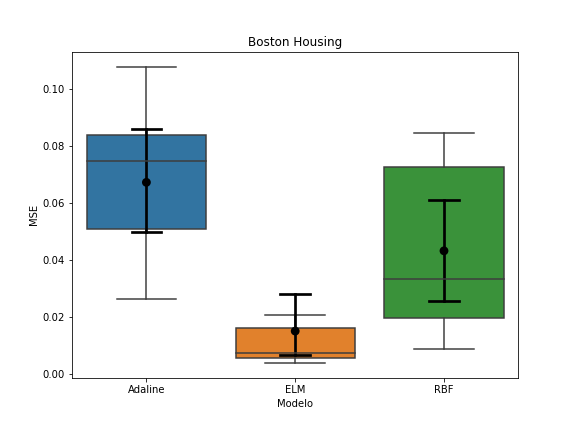
\includegraphics[width=0.5\textwidth]{figures/Boston Housing_scores.png}
%		\caption{Boxplots para a base de dados \textit{Boston Housing}. Intervalos de confiança de 95\% para a média são exibidos em preto.}
%		\label{fig:box-Boston-Housing}
%	\end{figure}
%	
%	\begin{figure}[thpbh]
%		\centering
%		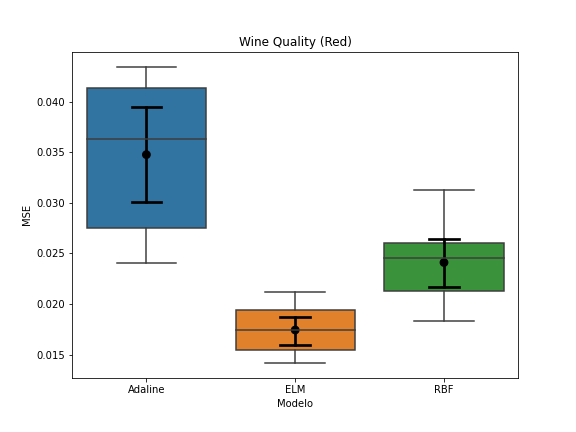
\includegraphics[width=0.5\textwidth]{figures/Wine Quality (Red)_scores.png}
%		\caption{Boxplots para a base de dados \textit{Wine Quality (Red)}. Intervalos de confiança de 95\% para a média são exibidos em preto.}
%		\label{fig:box-Wine}
%	\end{figure}
%	
%	\begin{figure}[thpbh]
%		\centering
%		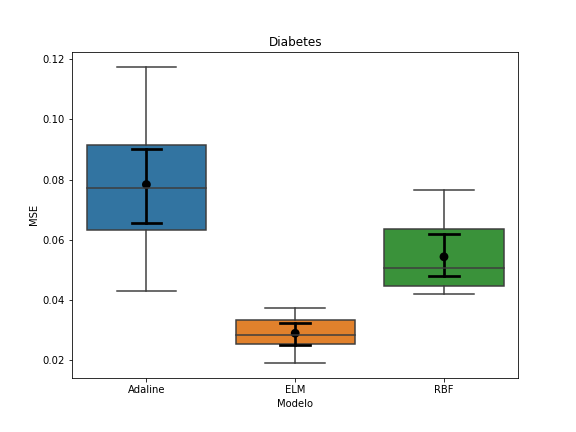
\includegraphics[width=0.5\textwidth]{figures/Diabetes_scores.png}
%		\caption{Boxplots para a base de dados \textit{Diabetes}. Intervalos de confiança de 95\% para a média são exibidos em preto.}
%		\label{fig:box-Diabetes}
%	\end{figure}


	
	\section{Conclusões}
	
	Neste trabalho foi feita uma avaliação do desempenho dos modelos ELM, RBF, Adaline, Perceptron e ELM Hebbiano sobre bases de dados de benchmark presentes na literatura. A partir de um experimento desenhado para tal finalidade, os resultados foram comparados estatísticamente utilizando a técnica de \textit{bootstrapping} para a média das métricas AUC e erro quadrático médio, considerando um intervalo de confiança de 95\%. Destaca-se o excelente desempenho do ELM em todos os conjuntos de dados, tanto de regressão e classificação. É importante destacar também o desempenho muito abaixo do esperado para o RBF nos problemas de classificação, sugerindo a necessidade de um melhor ajuste do número de neurônios na camada escondida, por exemplo. Notou-se também que os modelos lineares avaliados obtiveram bons resultados dependendo da base de dados em questão, conseguindo atingir um desempenho estatisticamente equivalente aos demais.
	
	Uma surpresa foi o ELM Hebbiano, onde embora tenha sido usada uma abordagem bem simples de aprendizado Hebbiano, não apresentou um resultado muito inferior em relação ao ELM original para classificação. Destaca-se o fato de que não foi possível utilizar a estratégia de aprendizado Hebbiano com sucesso em problemas de regressão. Isso sugere que uma abordagem diferente deve ser utilizada nesta situação. Durante a execução do experimento, pôde ser observado também que o modelo RBF possui um tempo de treinamento muito maior que os demais. Isso fez com que ele fosse o gargalo de todo o experimento neste quesito, o que limitou um pouco o potencial de executar um número maior de partições para a validação cruzada, bem como avaliar um intervalo maior para o fator de regularização. 
	
	Como trabalhos futuros, é sugerido um ajuste fino de demais hiper-parâmetros do RBF como forma de tentar melhorar o seu desempenho. Além disso, também é interessante avaliar outras formas de aprendizado Hebbiano que poderiam ser utilizados com o ELM, bem como para melhorar seu poder de generalização e também ser aplicável a problemas de regressão com sucesso. Outra tarefa importante seria a realização de uma etapa de pré-processamento mais completa sobre bases de dados considerados, o qual não foi feita por restrições de tempo mas teria potencial para melhorar os resultados obtidos de todos os modelos.
		


    \bibliographystyle{unsrt}
	\bibliography{artigo3}
	
\end{document} 